\documentclass[problem]{mcs}

\begin{pcomments}
  \pcomment{from: S09.ps5}
  \pcomment{from: F06.rec6 (revised by ARM)}
\end{pcomments}

\pkeywords{
  Euler_circuits
  cycles
  degree
}

%%%%%%%%%%%%%%%%%%%%%%%%%%%%%%%%%%%%%%%%%%%%%%%%%%%%%%%%%%%%%%%%%%%%%
% Problem starts here
%%%%%%%%%%%%%%%%%%%%%%%%%%%%%%%%%%%%%%%%%%%%%%%%%%%%%%%%%%%%%%%%%%%%%

\begin{problem}
  In this problem we'll consider some special cycles in graphs called {\em
    Euler circuits}, named after the famous mathematician Leonhard Euler.
  (Same Euler as for the constant $e\approx 2.718$ ---he did a lot of
  stuff.)

\begin{definition}
  An Euler circuit of a graph is a cycle which traverses every edge
  exactly once.
\end{definition}

Does the graph in the following figure contain an Euler circuit?

\begin{center}
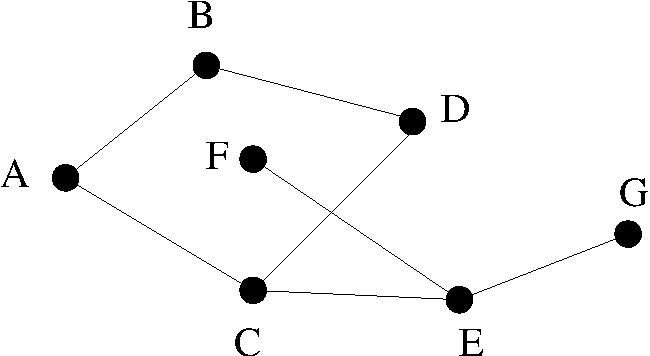
\includegraphics[height=1.75in]{example}
\end{center}

Well, if it did, the edge $(E, F)$ would need to be included.  If the path
does not start at $F$ then at some point it traverses edge $(E,F)$, and
now it is stuck at $F$ since $F$ has no other edges incident to it and an
Euler circuit can't traverse $(E,F)$ twice.  But then the path could not
be a circuit.  On the other hand, if the path starts at $F$, it must then
go to $E$ along $(E,F)$, but now it cannot return to $F$.  It again cannot
be a circuit. This argument generalizes to show that if a graph has a
vertex of degree $1$, it cannot contain an Euler circuit.

\iffalse
On the other hand, it is easy to see that any cycle contains an Euler
circuit. You can just start at any vertex and walk around back to it.
\fi

So how do you tell in general whether a graph has an Euler circuit?  At
first glance this may seem like a daunting problem (the similar sounding
problem of finding a cycle that touches every vertex exactly once is one
of those million dollar NP-complete problems known as the \term{Traveling
  Salesman Problem}) ---but it turns out to be easy.

\bparts

\ppart Show that if a graph has an Euler circuit, then the degree of each
of its vertices is even.

  \solution{Let circuit $C \eqdef v_1, v_2, \dots, v_r, v_1$ be an Euler
    circuit.  Consider any vertex $v$.  Then every time $v$ occurs in
    $C$, there is a vertex $a$ which comes immediately before $v$ and a
    vertex $b$ which comes immediately after $v$.  Note that this holds for
    $v = v_1$ as well since $C$ is a circuit. Moreover, $(a,v)$ and
    $(v,b)$ must be distinct edges of $G$ since $C$ is an Euler circuit.
    It follows that if $v$ occurs $s$ times in $C$, then it has degree
    $2s$ since every edge incident to $v$ occurs in $C$ exactly once.
    Thus, $v$ has even degree.}
\eparts

In the remaining parts, we'll work out the converse: if the degree of
every vertex of a connected finite graph is even, then it has an Euler
circuit.  To do this, let's define an Euler \term{path} to be a path that
traverses each edge \emph{at most} once.

\bparts

\ppart\label{conn} Suppose that an Euler path in a connected graph does
not traverse every edge.  Explain why there must be an untraversed edge
that is incident to a vertex on the path.

\solution{If either end of the untraversed edge is on the Euler path, that
  already is the desired edge.  So suppose there's an untraversed edge,
  $e$, both of whose endpoints are not on the Euler path.  Since the graph
  is connected, there must be a shortest path, $P$, from an endpoint of
  $e$ to a vertex on the Euler path.  Then all the edges on $P$ must be
  untraversed (or $P$ could be shortened), so the last edge traversed by
  $P$ will be the desired edge.}

\eparts

In the remaining parts, let $W$ be the \emph{longest} Euler path in some
finite, connected graph.

\bparts

\ppart\label{cycle-circuit} Show that if $W$ is a cycle, then it must be
an Euler circuit.

\hint part~\eqref{conn}

\solution{Suppose an edge was not traversed by $W$.  By part~\eqref{conn},
  there must be a vertex on $W$ incident to an edge not traversed by $W$.
  Starting at this vertex, go around $W$ back to that vertex, and then the
  follow the edge.  This makes a longer Euler path, contradicting the
  maximality of $W$.  So no edge can be missing from $W$.}

\ppart\label{already} Explain why all the edges incident to the end of $W$
must already have been traversed by $W$.

\solution{ Otherwise we could extend $W$ to a longer Euler path with any
  edge from the end not already traversed by $W$.  }

\ppart\label{odd} Show that if the end of $W$ was not equal to the start
of $W$, then the degree of the end would be odd.

\hint part~\eqref{already}

\solution{Let $v$ be the end vertex of $W$.  Given that $v$ is not the
  start of $W$, it follows that at any occurrence of $v$ in $W$ other than
  at the end, $W$ would enter and leave that occurrence of $v$ traversing
  a pair of edges.  Since $W$ is an Euler path, all the edges in all these
  pairs are distinct.  In addition, the final edge traversed by $W$ as it
  ends at $v$ is distinct from all the paired edges.  Altogether, this
  imples that there are an odd number of edges traversed by $W$ and
  incident to $v$.  But by part~\eqref{already}, these are all the edges
  incident to $v$, proving that $v$ has odd degree.}

\ppart Conclude that if every vertex of a finite, connected graph has even
degree, then it has an Euler circuit.

\solution{If all vertices in $G$ have even degree, then by
  part~\eqref{odd}, the only possibility is that the end of $W$ equals the
  start, that is, $W$ is a cycle.  So by part~\eqref{cycle-circuit}, $W$ is
  an Euler circuit.}

\eparts
\end{problem}

%%%%%%%%%%%%%%%%%%%%%%%%%%%%%%%%%%%%%%%%%%%%%%%%%%%%%%%%%%%%%%%%%%%%%
% Problem ends here
%%%%%%%%%%%%%%%%%%%%%%%%%%%%%%%%%%%%%%%%%%%%%%%%%%%%%%%%%%%%%%%%%%%%%
